\chapter{Arhitektura i dizajn sustava}		
	
	Sustav se može podijeliti na podsustave:
		\begin{packed_item}
			
			\item  Klijent
			\item  Poslužitelj
			\item  Baza podataka
			
		\end{packed_item}
	
		\begin{figure}[H]
			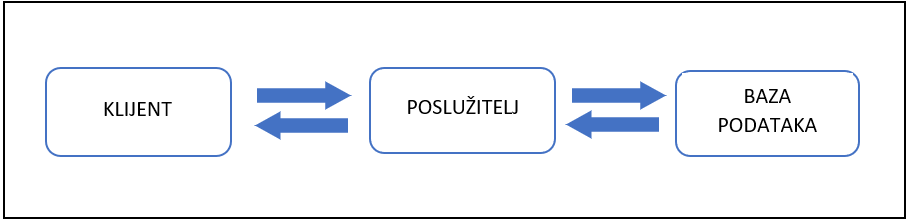
\includegraphics[width=\textwidth]{slike/Organizacija_sustava.PNG} %veličina u odnosu na širinu linije
			\caption{Organizacija sustava}
			\label{fig:organizacija_sustava1} %label mora biti drugaciji za svaku sliku
		\end{figure}
		
\underbar{\textit{Klijent}} 
Klijent je web preglednik pomoću kojeg korisnici pristupaju našoj web aplikaciji. Često korišteni web preglednici su: Google Chrome, Apple Safari, Mozilla Firefox. Kada korisnik pristupa web aplikaciji, web preglednik šalje HTTP (\textit{engl. Hypertext Transfer Protocol}) zahtjeve za preuzimanje statičkih datoteka web poslužitelju. Statičke datoteke mogu biti HTML, CSS i JavaScript datoteke koje sadrže React kod. Nakon preuzimanja datoteka, preglednik ih koristi za izgradnju i prikaz korisničkog sučelja te izvršavanje funkcija unutar aplikacije. 

\underbar{\textit{Poslužitelj}} 
Poslužitelj je Python kod pisan unutar web mikrookvira Flask. On služi kao posrednik između  klijenta (korisničkog sučelja) i baze podataka. U Python kodu (Flask aplikaciji) definirani su RESTful API-ji (kao rute ili krajnje točke) koji omogućuju klijentima da šalju HTTP zahtjeve za određene podatke. Prilikom obrade tih zahtjeva, Python kod šalje upite bazi podataka kako bi dohvatio, promijenio ili dodao tražene podatke.

\underbar{\textit{Baza podataka}}
Kada baza podataka zaprimi upite od poslužitelja, ona ih izvršava i vraća rezultate poslužitelju. Vraćeni rezultati mogu biti u obliku potvrde o izvršenom upitu ili u obliku podataka koje je poslužitelj zatražio od baze podataka. Baza podataka ostaje pasivna sve dok ne zaprimi nove upite od poslužitelja.

Aplikacije je organizirana po MVC (\textit{engl. Model-View-Controller}, hrv. Model-Pogled-Nadglednik) obrascu.  

Općenito, \underbar{\textit{Model}} definira podatke, njihovu strukturu i operacije koje se mogu izvršavati nad tim podacima. \underbar{\textit{Pogled}} predstavlja prikaz podataka korisniku (npr. korisničko sučelje). \underbar{\textit{Nadglednik}} predstavlja posrednike između Modela i Nadglednika. Oni obrađuju zahtjeve korisnika, vrše operacije nad Modelom i ažuriraju Pogled. Organizacijom prema ovom obrascu olakšava se proširivanje i održavanje aplikacije.

Naša aplikacija ne sadrži doslovno sve tri navedene komponente. Ovdje Python objedinjuje Model i dio logike Nadglednika. Komponente u React-u odgovaraju Pogledu te je i ovdje sadržan dio logike Nadglednika.

				
		\section{Baza podataka}

Za rješavanje projektnog zadatka odabrana je relacijska baza podataka. Implementirali smo je korištenjem sustava PostgreSQL. To je besplatan sustav za upravljanje bazom podataka otvorenog koda. Objekti relacijske baze podataka su relacije. Neformalno, i u PostgreSQL-u, to su dvodimenzionalne imenovane tablice gdje imenovani stupac predstavlja atribut, a redak zapis relacije. Izbor ovakve baze podataka omogućio nam je lakše strukturiranje podatka i definiranje veza između njih, normalizaciju, skalabilnost te sigurnost kod pohrane i dohvata podataka. 
Zbog potreba naše aplikacije, baza podataka sadrži entitete:

        \begin{packed_item}
		\item 	\textnormal{Korisnik}
		\item 	\textnormal{Djelatnik}
		\item 	\textnormal{Uloga}
        \item 	\textnormal{Pacijent}
        \item 	\textnormal{Terapija}
        \item 	\textnormal{VrstaTerapije}	
        \item 	\textnormal{Termin}			
        \item 	\textnormal{Status}	
        \item 	\textnormal{Oprema}
        \item 	\textnormal{ZauzetaOprema}	
        \item 	\textnormal{Soba}	
        \item 	\textnormal{Uredaj}
        \item 	\textnormal{VrstaUredaja}
                   				
	 \end{packed_item}

		
			\subsection{Opis tablica}
			
 \textbf{Korisnik:}

 \textnormal{Entitet Korisnik sadrži sve bitne informacije o korisniku aplikacije. Entitet sadrži atribute: idKorisnika, ime, prezime, datumRodenja, adresa, email, lozinka. Korisnik može biti ili djelatnik zdravstvene ustanove ili pacijent koji se želi naručiti na terapiju u zdravstvenoj ustanovi.}

				
				
				\begin{longtblr}[
					label=none,
					entry=none
					]{
						width = \textwidth,
						colspec={|X[6,l]|X[7, l]|X[20, l]|}, 
						rowhead = 1,
					} %definicija širine tablice, širine stupaca, poravnanje i broja redaka naslova tablice
					\hline \SetCell[c=3]{c}{\textbf{Korisnik}}	 \\ \hline[3pt]
					\SetCell{LightGreen}idKorisnika & INT & jedinstveni identifikator korisnika 	\\ \hline
					ime & VARCHAR(50) & ime korisnika	\\ \hline 
                                               prezime & VARCHAR(50) & prezime korisnika	\\ \hline
                                               datumRodenja & DATE & datum rođenja korisnika	\\ \hline  
                                               adresa & VARCHAR(100) & adresa mjesta stanovanja korisnika	\\ \hline 
					 email & VARCHAR(50) & e-mail adresa korisnika   \\ \hline 
					 lozinka & VARCHAR(50) & hash lozinke za prijavu u aplikaciju	\\ \hline 
					 
				\end{longtblr}

\textbf{Djelatnik:}

\textnormal{Entitet Djelatnik je ekskluzivna specijalizacija entiteta Korisnik. Entitet sadrži atribute: idKorisnika, aktivan, idUloge.}

				\begin{longtblr}[
					label=none,
					entry=none
					]{
						width = \textwidth,
						colspec={|X[6,l]|X[7, l]|X[20, l]|}, 
						rowhead = 1,
					} %definicija širine tablice, širine stupaca, poravnanje i broja redaka naslova tablice
					\hline \SetCell[c=3]{c}{\textbf{Djelatnik}}	 \\ \hline[3pt]
					\SetCell{LightBlue}idKorisnika & INT & jedinstveni identifikator korisnika (korisnik.idKorisnika) 	\\ \hline
					aktivan & CHAR(2) & označava radni odnos liječnika i zdravstvene ustanove	\\ \hline 
					\SetCell{LightBlue}idUloge & INT & jedinstveni identifikator uloge (uloga.idUloge)	\\ \hline 
					 
				\end{longtblr}

\textbf{Uloga:}

\textnormal{Entitet Uloga služi za razlikovanje djelatnika zdravstvene ustanove. U aplikaciji razlikujemo liječnike od administratora. Entitet sadrži atribute: idUloge, imeUloge.}

				\begin{longtblr}[
					label=none,
					entry=none
					]{
						width = \textwidth,
						colspec={|X[6,l]|X[7, l]|X[20, l]|}, 
						rowhead = 1,
					} %definicija širine tablice, širine stupaca, poravnanje i broja redaka naslova tablice
					\hline \SetCell[c=3]{c}{\textbf{Uloga}}	 \\ \hline[3pt]
					\SetCell{LightGreen}idUloge & INT & jedinstveni identifikator uloge 	\\ \hline
					imeUloge & VARCHAR(50) & naziv uloge (liječnik ili administrator)	\\ \hline 
					 
				\end{longtblr}

\textbf{Pacijent:}

\textnormal{Entitet Pacijent je ekskluzivna specijalizacija entiteta Korisnik. Entitet sadrži atribute: idKorisnika, MBO.}

				\begin{longtblr}[
					label=none,
					entry=none
					]{
						width = \textwidth,
						colspec={|X[6,l]|X[7, l]|X[20, l]|}, 
						rowhead = 1,
					} %definicija širine tablice, širine stupaca, poravnanje i broja redaka naslova tablice
					\hline \SetCell[c=3]{c}{\textbf{Pacijent}}	 \\ \hline[3pt]
					\SetCell{LightBlue}idKorisnika & INT & jedinstveni identifikator korisnika (korisnik.idKorisnika)	\\ \hline
					MBO & CHAR(9) & matični broj osiguranika (pacijenta)	\\ \hline 

					 
				\end{longtblr}

\textbf{Terapija:}

\textnormal{Entitet Terapija sadrži sve bitne informacije o terapiji na koju je pacijent naručen. Entitet sadrži atribute: idTerapije, idLijecnika, opisOboljenja, zahtPostLijec, datumPoc, datumZavrs, idPacijenta, idDjelatnika, idVrste.}

				\begin{longtblr}[
					label=none,
					entry=none
					]{
						width = \textwidth,
						colspec={|X[6,l]|X[7, l]|X[20, l]|}, 
						rowhead = 1,
					} %definicija širine tablice, širine stupaca, poravnanje i broja redaka naslova tablice
					\hline \SetCell[c=3]{c}{\textbf{Terapija}}	 \\ \hline[3pt]
					\SetCell{LightGreen}idTerapije & INT & jedinstveni identifikator terapije	\\ \hline
					idLijecnika & INT & jedinstveni identifikator liječnika	\\ \hline 
                    opisOboljenja & VARCHAR(200) & opis oboljenja pacijenta	\\ \hline
                    zahtPostLijec & VARCHAR(200) & zahtjev za postupkom liječenja (terapijom)	\\ \hline  
                    datumPoc & DATE & datum početka terapije	\\ \hline 
					 datumZavrs & DATE & datum završetka terapije   \\ \hline 
					 \SetCell{LightBlue}idPacijenta & INT & jedinstveni identifikator pacijenta (korisnik.idKorisnika)	\\ \hline 
					 \SetCell{LightBlue}idDjelatnika & INT & jedinstveni identifikator djelatnika (korisnik.idKorisnika) \\ \hline
					 \SetCell{LightBlue}idVrste & INT & jedinstveni identifikator vrste uređaja (vrstaTerapije.idVrste) \\ \hline
					 
				\end{longtblr}

\textbf{VrstaTerapije:}

Entitet VrstaTerapije sadrži sve bitne informacije o vrsti terapije na koju je pacijent naručen. Entitet sadrži atribute: idVrste, imeVrste, opisVrste.

\begin{longtblr}[
					label=none,
					entry=none
					]{
						width = \textwidth,
						colspec={|X[6,l]|X[7, l]|X[20, l]|}, 
						rowhead = 1,
					} %definicija širine tablice, širine stupaca, poravnanje i broja redaka naslova tablice
					\hline \SetCell[c=3]{c}{\textbf{VrstaTerapije}}	 \\ \hline[3pt]
					\SetCell{LightGreen}idVrste & INT & jedinstveni identifikator vrste terapije	\\ \hline
					imeVrste & VARCHAR(50) & naziv vrste terapije	\\ \hline 
                                               opisVrste & VARCHAR(200) & opis vrste terapije	\\ \hline
					 
				\end{longtblr}

\textbf{Termin:}

\textnormal{Entitet Termin sadrži sve bitne informacije o terminu terapije na koji je pacijent naručen. Entitet Termin ne postoji bez entiteta vlasnika, entiteta Terapija. (Termin je egzistencijalno slab entitet.)}

\begin{longtblr}[
					label=none,
					entry=none
					]{
						width = \textwidth,
						colspec={|X[6,l]|X[7, l]|X[20, l]|}, 
						rowhead = 1,
					} %definicija širine tablice, širine stupaca, poravnanje i broja redaka naslova tablice
					\hline \SetCell[c=3]{c}{\textbf{Termin}}	 \\ \hline[3pt]
					\SetCell{LightGreen}idTermina & INT & jedinstveni identifikator termina terapije \\ \hline
					\SetCell{LightBlue}idTerapije & INT & jedinstveni identifikator terapije (terapija.idTerapije)	\\ \hline 
                                               od & DATETIME & datum i vrijeme početka termina	\\ \hline
					 do & DATETIME & datum i vrijeme završetka termina      \\ \hline
                                               komentar & VARCHAR(200) & komentar liječnika o napretku terapije \\ \hline
                                               \SetCell{LightBlue}brSobe & VARCHAR(10) & jedinstveni identifikator sobe (soba.brSobe)	\\ \hline
                                               \SetCell{LightBlue}idStatus & INT & jedinstveni identifikator statusa (status.idStatus)	\\ \hline
                                               \SetCell{LightBlue}idKorisnika & INT & jedinstveni identifikator korisnika (korisnik.idKorisnika)	\\ \hline
				\end{longtblr}

\textbf{Soba:}

\textnormal{Entitet Soba sadrži sve bitne informacije o sobi u kojoj se provodi neka terapija. Entitet sadrži atribute: brSobe, kapacitet.}

\begin{longtblr}[
					label=none,
					entry=none
					]{
						width = \textwidth,
						colspec={|X[6,l]|X[7, l]|X[20, l]|}, 
						rowhead = 1,
					} %definicija širine tablice, širine stupaca, poravnanje i broja redaka naslova tablice
					\hline \SetCell[c=3]{c}{\textbf{Soba}}	 \\ \hline[3pt]
					\SetCell{LightGreen}brSobe & VRACHAR(10) & jedinstveni identifikator sobe \\ \hline
                                               kapacitet & INT & kapacitet sobe, broj pacijenata koji istovremeno mogu biti na terapiji u nekoj sobi	\\ \hline
				\end{longtblr}

\textbf{Uredaj:}

\textnormal{Entitet Uredaj sadrži sve bitne informacije o uređaju koji se koristi u nekoj terapiji. Entitet sadrži atribute: idUredaja, brSobe, idVrste.}

\begin{longtblr}[
					label=none,
					entry=none
					]{
						width = \textwidth,
						colspec={|X[6,l]|X[7, l]|X[20, l]|}, 
						rowhead = 1,
					} %definicija širine tablice, širine stupaca, poravnanje i broja redaka naslova tablice
					\hline \SetCell[c=3]{c}{\textbf{Uredaj}}	 \\ \hline[3pt]
					\SetCell{LightGreen}idUredaja & INT & jedinstveni identifikator uređaja \\ \hline
                                               \SetCell{LightBlue}brSobe & VARCHAR(10) & jedinstveni identifikator sobe (soba.brSobe) \\ \hline
                                               \SetCell{LightBlue}idVrste & INT & jedinstveni identifikator vrste uređaja (vrstaUredaja.idVrste)\\ \hline
				\end{longtblr}

\textbf{VrstaUredaja:}

\textnormal{Entitet VrstaUredaja sadrži sve bitne informacije o vrsti uređaja koja se primijenjuje u nekoj terapiji. Entitet sadrži atribute: idVrste, imeVrste, opisVrste.}

\begin{longtblr}[
					label=none,
					entry=none
					]{
						width = \textwidth,
						colspec={|X[6,l]|X[7, l]|X[20, l]|}, 
						rowhead = 1,
					} %definicija širine tablice, širine stupaca, poravnanje i broja redaka naslova tablice
					\hline \SetCell[c=3]{c}{\textbf{VrstaUredaja}}	 \\ \hline[3pt]
					\SetCell{LightGreen}idVrste & INT & jedinstveni identifikator vrste uređaja \\ \hline
                                               imeVrste & VARCHAR(50) & naziv vrste uređaja \\ \hline
                                               opisVrste & VARCHAR(200) & opis vrste uređaja \\ \hline
				\end{longtblr}

\textbf{Oprema:}

\textnormal{Entitet Oprema sadrži sve bitne informacije o opremi koja je na raspolaganju u zdravstvenoj ustanovi. Entitet sadrži atribute: idOpreme, imeOpreme, opisOpreme.}

\begin{longtblr}[
					label=none,
					entry=none
					]{
						width = \textwidth,
						colspec={|X[6,l]|X[7, l]|X[20, l]|}, 
						rowhead = 1,
					} %definicija širine tablice, širine stupaca, poravnanje i broja redaka naslova tablice
					\hline \SetCell[c=3]{c}{\textbf{Oprema}}	 \\ \hline[3pt]
					\SetCell{LightGreen}idOpreme & INT & jedinstveni identifikator opreme \\ \hline
                                               imeOpreme & VARCHAR(50) & naziv opreme (npr. štake)\\ \hline
                                               opisOpreme & VARCHAR(200) & opis namjene opreme \\ \hline
				\end{longtblr}

\textbf{ZauzetaOprema:}

\textnormal{Entitet ZauzetaOprema sadrži sve bitne informacije o alokaciji opreme po terminima. Entitet sadrži atribute: idTermina, idTerapije, idOpreme.}

\begin{longtblr}[
					label=none,
					entry=none
					]{
						width = \textwidth,
						colspec={|X[6,l]|X[7, l]|X[20, l]|}, 
						rowhead = 1,
					} %definicija širine tablice, širine stupaca, poravnanje i broja redaka naslova tablice
					\hline \SetCell[c=3]{c}{\textbf{ZauzetaOprema}}	 \\ \hline[3pt]
					\SetCell{LightBlue}idTermina & INT & jedinstveni identifikator termina (termin.idTermina) \\ \hline
                                               \SetCell{LightBlue}idTerapije & INT & jedinstveni identifikator terapije (terapija.idTerapije) \\ \hline
                                               \SetCell{LightBlue}idOpreme & INT & jedinstveni identifikator opreme (oprema.idOpreme)  \\ \hline
				\end{longtblr}

\textbf{Status:}

\textnormal{Entitet Status sadrži sve bitne informacije o statusu termina terapija koji je dodijeljen nekom pacijentu. Entitet sadrži atribute: idStatus, imeStatus.}

\begin{longtblr}[
					label=none,
					entry=none
					]{
						width = \textwidth,
						colspec={|X[6,l]|X[7, l]|X[20, l]|}, 
						rowhead = 1,
					} %definicija širine tablice, širine stupaca, poravnanje i broja redaka naslova tablice
					\hline \SetCell[c=3]{c}{\textbf{Status}}	 \\ \hline[3pt]
					\SetCell{LightGreen}idStatus & INT & jedinstveni identifikator uređaja \\ \hline
                                               imeStatus & VARCHAR(50) & naziv statusa (npr. u tijeku, završen...) \\ \hline
     
				\end{longtblr}	
				
			
			\subsection{Dijagram baze podataka}
		\begin{figure}[H]
			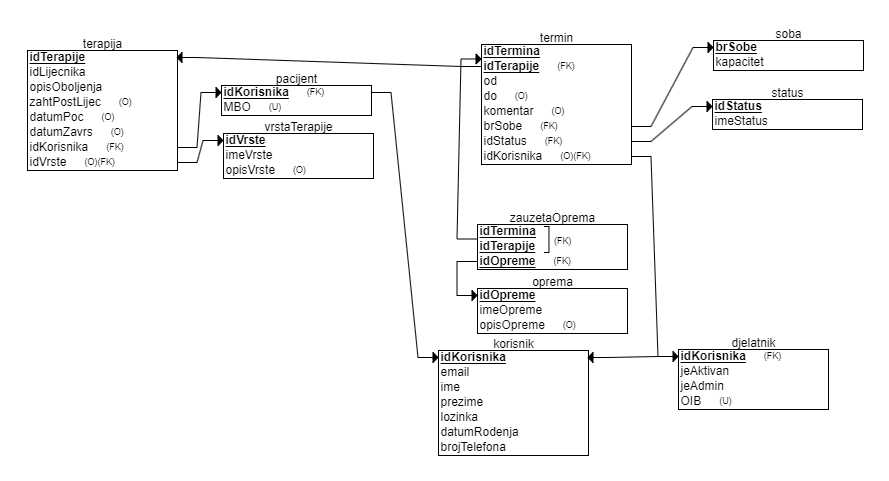
\includegraphics[width=\textwidth]{slike/Relacijska_shema.PNG} %veličina u odnosu na širinu linije
			\caption{Relacijska shema baze podataka}
			\label{fig:relacijska_shema1} %label mora biti drugaciji za svaku sliku
		\end{figure}
			
		\section{Dijagram razreda}
		
			\textit{Potrebno je priložiti dijagram razreda s pripadajućim opisom. Zbog preglednosti je moguće dijagram razlomiti na više njih, ali moraju biti grupirani prema sličnim razinama apstrakcije i srodnim funkcionalnostima.}\\
			
			\textbf{\textit{dio 1. revizije}}\\
			
			\textit{Prilikom prve predaje projekta, potrebno je priložiti potpuno razrađen dijagram razreda vezan uz \textbf{generičku funkcionalnost} sustava. Ostale funkcionalnosti trebaju biti idejno razrađene u dijagramu sa sljedećim komponentama: nazivi razreda, nazivi metoda i vrste pristupa metodama (npr. javni, zaštićeni), nazivi atributa razreda, veze i odnosi između razreda.}\\
			
			\textbf{\textit{dio 2. revizije}}\\			
			
			\textit{Prilikom druge predaje projekta dijagram razreda i opisi moraju odgovarati stvarnom stanju implementacije}
			
			
			
			\eject
		
		\section{Dijagram stanja}
			
			
			\textbf{\textit{dio 2. revizije}}\\
			
			\textit{Potrebno je priložiti dijagram stanja i opisati ga. Dovoljan je jedan dijagram stanja koji prikazuje \textbf{značajan dio funkcionalnosti} sustava. Na primjer, stanja korisničkog sučelja i tijek korištenja neke ključne funkcionalnosti jesu značajan dio sustava, a registracija i prijava nisu. }
			
			
			\eject 
		
		\section{Dijagram aktivnosti}
			
			\textbf{\textit{dio 2. revizije}}\\
			
			 \textit{Potrebno je priložiti dijagram aktivnosti s pripadajućim opisom. Dijagram aktivnosti treba prikazivati značajan dio sustava.}
			
			\eject
		\section{Dijagram komponenti}
		
			\textbf{\textit{dio 2. revizije}}\\
		
			 \textit{Potrebno je priložiti dijagram komponenti s pripadajućim opisom. Dijagram komponenti treba prikazivati strukturu cijele aplikacije.}